\section{Concept of execution}

Figure \ref{fig:sekvens1} shows the concept of execution among the system components. It shows the dynamic relationship of the components, that is, how they will interact during system operation. The diagram is based on the overall functionality of the system. 


\begin{figure}[H]
\centering
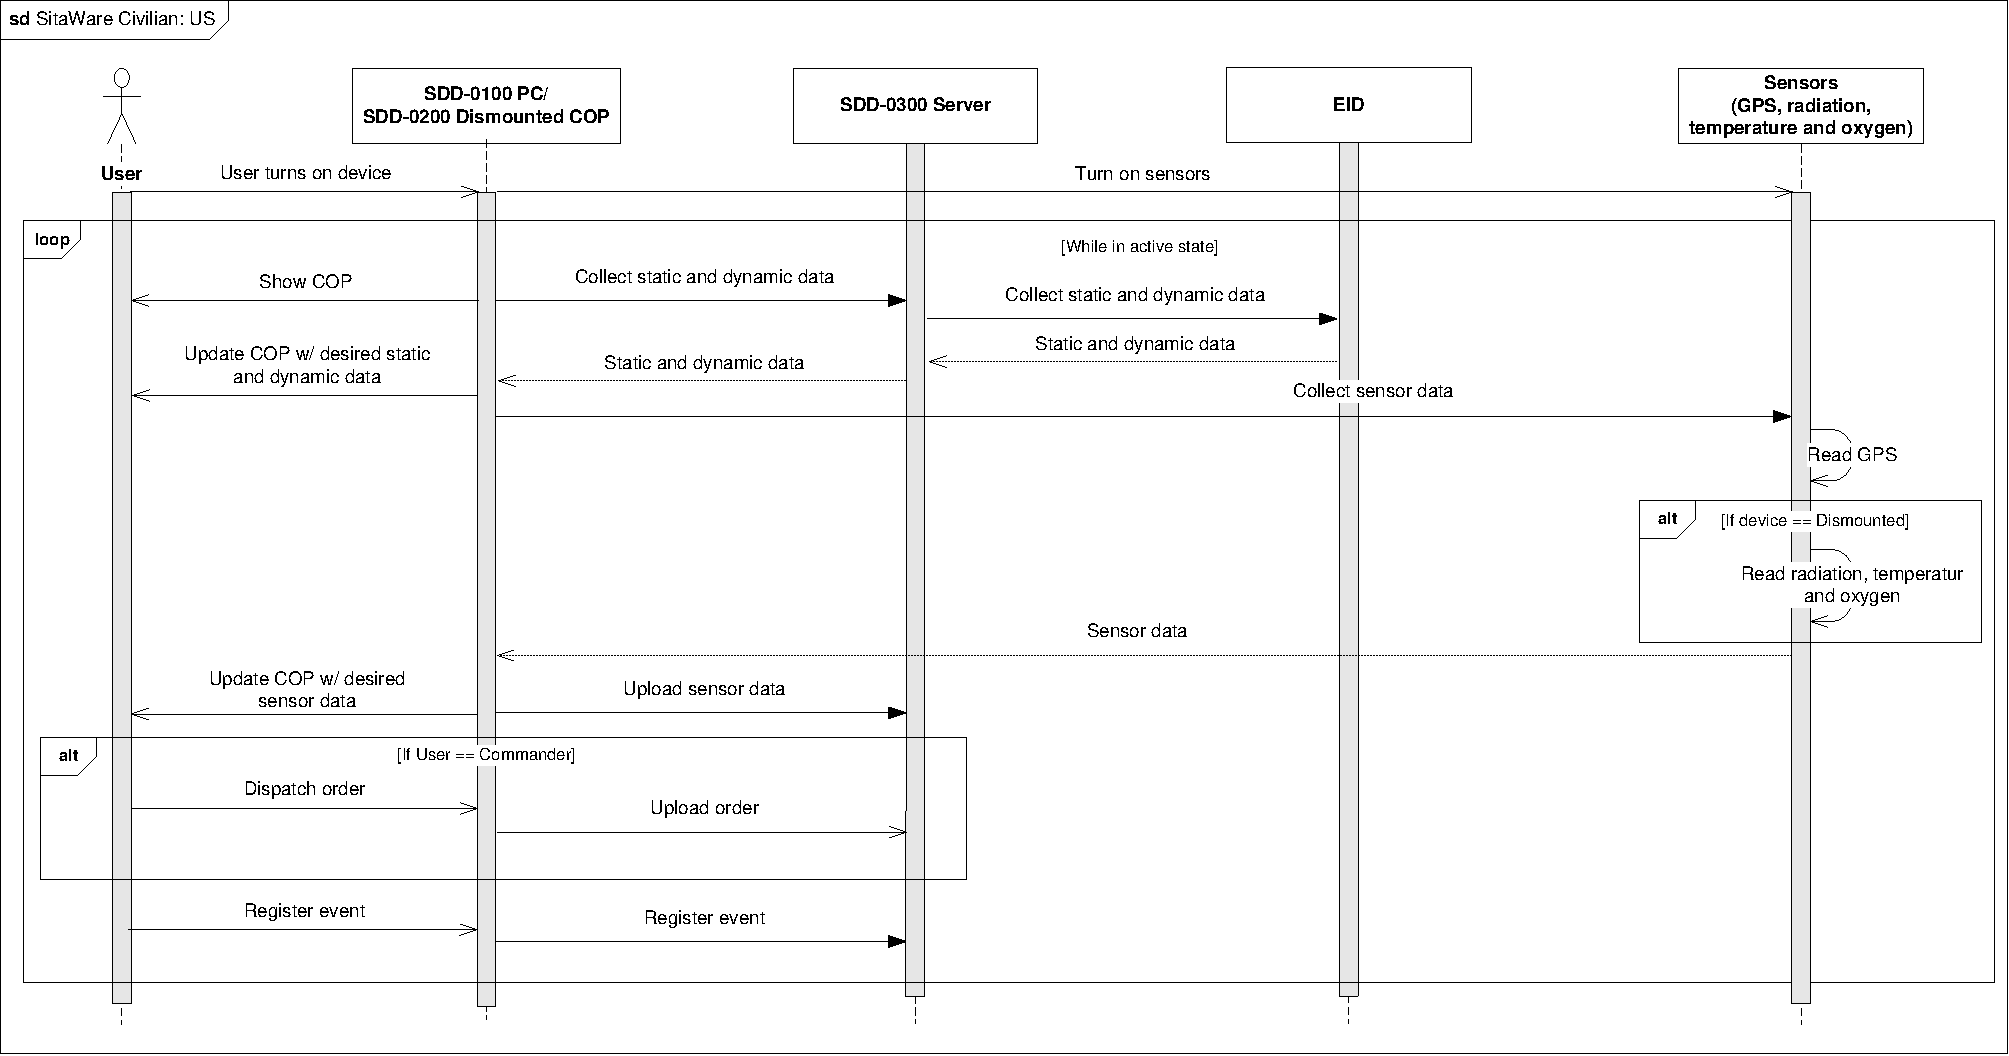
\includegraphics[width=0.95\textwidth]
{billeder/sekvens1.pdf}
\caption{Overall sequence diagram for SitaWare Civilian.}
\label{fig:sekvens1}
\end{figure}

Figure \ref{fig:stateDiagram} shows how the system executes through it's different states. Furthermore the different modes are shown. Which mode is used is determined by what user rights the user has.

\begin{figure}[H]
\centering
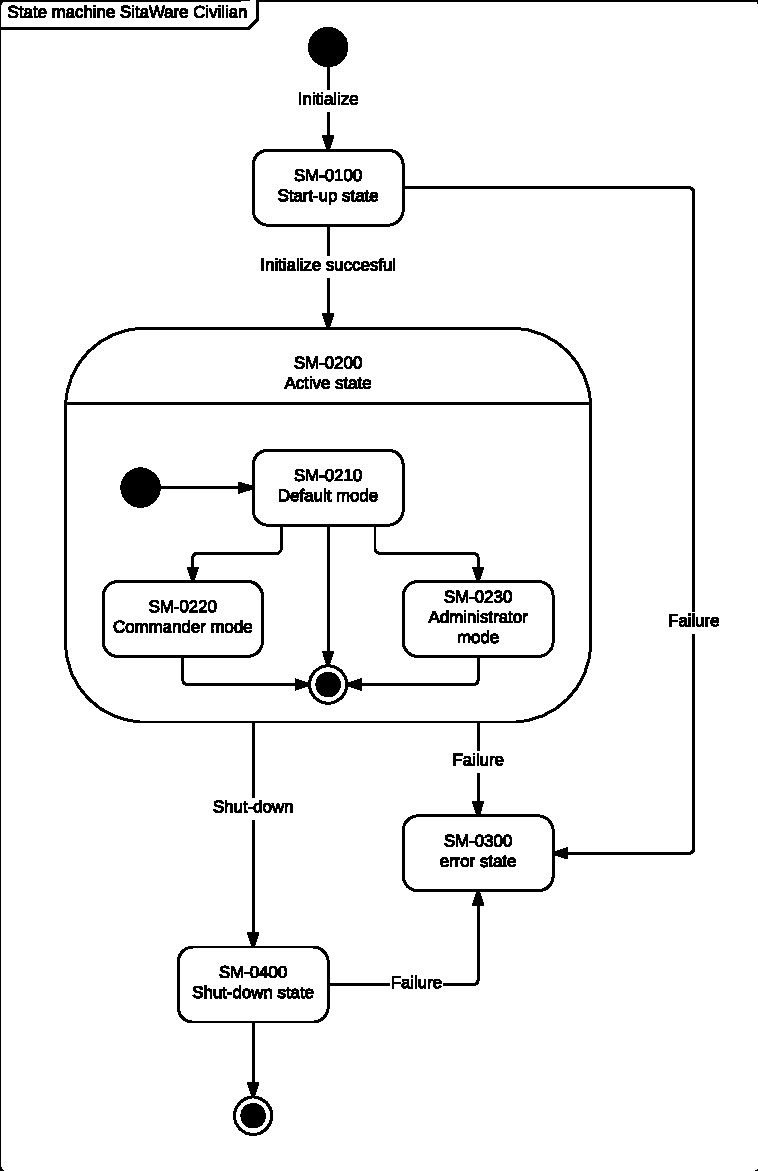
\includegraphics[width=0.95\textwidth]
{billeder/State_machine_PDD.pdf}
\caption{State diagram for SitaWare Civilian.}
\label{fig:stateDiagram}
\end{figure}